\documentclass{article}
\usepackage{nips15submit_e,times}
\usepackage{latexsym}
% \setlength\titlebox{5cm}    % Expanding the titlebox

%%% Custom additions %%%
% \usepackage{hyperref}
\usepackage{url}
\usepackage[leqno, fleqn]{amsmath}
\usepackage{amssymb}
\usepackage{qtree}
\usepackage{graphicx}
\usepackage{booktabs}
\usepackage{colortbl}
\usepackage{caption}
\usepackage{subcaption}
\usepackage{xcolor}
\usepackage{color}
\usepackage{tikz}
\usepackage{todonotes}
\usepackage[numbers]{natbib}

\newcount\colveccount
\newcommand*\colvec[1]{
        \global\colveccount#1
        \begin{bmatrix}
        \colvecnext
}
\def\colvecnext#1{
        #1
        \global\advance\colveccount-1
        \ifnum\colveccount>0
                \\
                \expandafter\colvecnext
        \else
                \end{bmatrix}
        \fi
}


\newcommand{\nateq}{\equiv}
\newcommand{\natind}{\mathbin{\#}}
%\newcommand{\natneg}{\raisebox{2px}{\tiny\thinspace$\wedge$\thinspace}}
\newcommand{\natneg}{\mathbin{^{\wedge}}}
\newcommand{\natfor}{\sqsubset}
\newcommand{\natrev}{\sqsupset}
\newcommand{\natalt}{\mathbin{|}}
\newcommand{\natcov}{\mathbin{\smallsmile}}

\newcommand{\qq}{\hspace{0.1em}}
\newcommand{\plneg}{\mathop{\textit{not}\qq}}
\newcommand{\pland}{\mathbin{\qq\textit{and}\qq}}
\newcommand{\plor}{\mathbin{\qq\textit{or}\qq}}




% Strikeout
\newlength{\howlong}\newcommand{\strikeout}[1]{\settowidth{\howlong}{#1}#1\unitlength0.5ex%
\begin{picture}(0,0)\put(0,1){\line(-1,0){\howlong\divide\unitlength}}\end{picture}}

\newcommand{\True}{\texttt{T}}
\newcommand{\False}{\texttt{F}}
\usepackage{stmaryrd}
\newcommand{\sem}[1]{\ensuremath{\llbracket#1\rrbracket}}

\newcommand{\mynote}[1]{{\color{blue}#1}}

\newcommand{\tbchecked}[1]{{\color{red}#1}}

\usepackage{gb4e}
\noautomath

\def\ii#1{\textit{#1}}
\newcommand{\word}[1]{\emph{#1}}
\newcommand{\newcite}[1]{\cite{#1}}

%%% %%%

\title{Tree-Structured Composition in Neural Networks\\without Tree-Structured Architectures}

% TODO: Make sure setup doesn't prime equal performance

%\Thanks{}}

\author{
Samuel R.\ Bowman, Christopher D. Manning, and Christopher Potts\\
Stanford University\\
Stanford, CA 94305-2150\\
\texttt{\{sbowman, manning, cgpotts\}@stanford.edu} \\
}


\date{}

\makeatletter
\newcommand{\@BIBLABEL}{\@emptybiblabel}
\newcommand{\@emptybiblabel}[1]{}
\definecolor{black}{rgb}{0,0,0}
\makeatother
\usepackage[breaklinks, draft, colorlinks, linkcolor=black, urlcolor=black, citecolor=black]{hyperref}

\nipsfinalcopy

\begin{document}
\maketitle

\begin{abstract}
Tree-structured neural networks aim to deliver a robust and principled method for representing sentence meaning, but these models largely have not outperformed simpler sequence-based models by substantial margins. We hypothesize that sequence models like LSTMs are able to discover and implicitly use the same kinds of recursive compositional structures that the tree-structured ones are built around---at least in cases where there are clear cues to that structure in the data---mitigating the advantage of the tree-structured models. We investigate this possibility by evaluating both models on an artificial task for which recursive compositional structure is crucial, and find that the sequence model is able to exploit the underlying structure, though it is less efficient at learning than the tree models, only succeeding after exposure to a larger and richer set of training data.
\end{abstract}

\section{Introduction}\label{sec:introduction}

The semantic concepts of entailment and contradiction are central to
all aspects of natural language meaning
\cite{Katz72,vanBenthem08NATLOG}, from the lexicon to the content of
entire texts. Thus, \emph{natural language
  inference} (NLI) --- characterizing and using these relations in
computational systems
\cite{dagan2006pascal,MacCartney09,maccartney2009extended} --- is
essential in tasks ranging from information retrieval to semantic
parsing to commonsense reasoning.

NLI has been addressed using a wide variety of techniques, including
those grounded in syntactic structures, knowledge bases, and symbolic
logic. In recent years, it has become an important testing ground for
approaches employing \emph{distributed} word and phrase
representations. Distributed representations excel at capturing
relations based in similarity, but it is less clear that they can be
trained to support the full range of logical inferences required for
NLI. In the SemEval 2014 task aimed at evaluating distributed
representations for NLI, the best-performing systems relied heavily on
additional features and reasoning capabilities
\cite{marelli2014semeval}.

Our primary objective in this paper is to provide a new empirical
evaluation of a wide range of models for distributed semantic
representations in the context of NLI. However, in our view, the
existing corpus resources in this area do not permit such an
assessment. They are generally too small for training modern
data-intensive, wide-coverage models, and they are often beset with
indeterminacies of event and entity coreference that significantly
impact annotation quality.

To address this, we present a new corpus of sentence pairs labeled for
entailment, contradiction, and semantic independence. At 550,152
sentence-pairs, this corpus is orders of magnitude larger than all
other resources of its type. And, in contrast to many such resources,
all of the sentences were written by humans in a grounded,
naturalistic context. In a separate validation phase, we collected
four additional judgments for each label for 56,941 of the examples,
and 98\% of cases emerge with a gold label, which attests to the high
quality of the data.

In this paper, we use this corpus to evaluate a wide variety of models
for natural language inference, including rule-based systems, simple
linear classifiers, and compositional neural networks. We find that
Tree-Structured Long Short-Term Memory networks (TreeLSTMs;
\citealt{tai2015improved,le2015compositional}) achieve the best
performance. In addition, we enhance the case for TreeLSTMs by showing
that its representations, trained on our corpus, perform well in a
disparate set of additional semantic tasks.  The success of these
transfer-learning experiments is also a testament to the centrality
of NLI in semantics.


%%%%%%%%%%%%%%%%%%%%%%%%%%%%%%%%%%%%%%%%%%%%%%%%%%%%%%%%%%%%%%%%%%%%%%


% One point of comparison that might be good to set up (maybe not in these words, this is Sam's sketch):

% Translation can also be used to train/evaluate NNs, and also demands some degree of sensitivity to compositional syntactic and semantic structure. Plus, it's easier to get good data for that task. But NLI is the better benchmark for developing NNs for language understanding, because:

% (i) Typical translation tasks require natural language generation, which is a separate difficult problem that must be learned in parallel with the semantic encoding task of interest, making results harder to interpret. We can just a vanilla well-understood classifier on top of our sentence model.

% (ii) Contradiction vs. entailment decisions in particular specifically target the abilities of NN models to learn lexical and phrasal representations (like alternation) that don't resemble similarity, either in their correlation with distributional information or their transitivity behavior. MT doesn't seem to have a good parallel to this. Since modeling similarity is almost the only aspect of NN behavior in NLP that's reasonably well understood and basically known to work, using a benchmark that explicitly demands something more sophisticated than this is likely to pay off by better exposing the weaknesses of current standard models.

% It might be also worth making an explicit comparison with sentiment as a benchmark, but that's low-hanging fruit.
\section{Recursive structure in artificial data}\label{sec:recursion}
\paragraph{Reasoning about entailment} 
The data that we use define a version of the \emph{recognizing textual entailment} task, in which the goal is to determine what kind of logical consequence relation holds between two sentences, drawing on a small fixed vocabulary of relations such as entailment, contradiction, and synonymy. This task is well suited to evaluating neural network models for sentence interpretation: models must develop comprehensive representations of the meanings of each sentence to do well at the task, but the data do not force these representations to take a specific form, allowing the model to learn whatever kind of representations it can use most effectively.

The data we use are labeled with the seven mutually exclusive logical relations of \newcite{maccartney2009extended}, which distinguish entailment in two directions ($\natfor$, $\natrev$), equivalence ($\nateq$), exhaustive and non-exhaustive contradiction ($\natneg$, $\natalt$), and two types of semantic independence ($\natind$, $\natcov$).

%\begin{table}[tp]
%  \centering\small
%  \renewcommand{\arraystretch}{1}
%  \begin{tabular}{l c l l} 
%    \toprule
%    Name & Symb. & Set-theoretic definition \\ 
%    \midrule
%strict entailment         & $\natfor$   & $x \subset y$  \\ 
%    strict rev. entailment & $\natrev$   & $x \supset y$  \\ 
%    equivalence        & $\nateq$    & $x = y$   \\ 
%    alternation        & $\natalt$   & $x \cap y = \emptyset \wedge x \cup y \neq \mathcal{D}$ \\ 
%    negation           & $\natneg$   & $x \cap y = \emptyset \wedge x \cup y = \mathcal{D}$   \\
%    cover              & $\natcov$   & $x \cap y \neq \emptyset \wedge x \cup y = \mathcal{D}$ \\ 
%    independence       & $\natind$   & (else)\\
%    \bottomrule
%  \end{tabular}
%  \caption{\label{b-table}MacCartney's seven mutually exclusive relations are defined abstractly on pairs of sets drawing from the universe $\mathcal{D}$, but can be straightforwardly applied to any pair of natural language words, phrases, or sentences.
%  } %-%
%\end{table}

\begin{table}[tp]
  \centering\small
%  \begin{subtable}[t]{0.45\textwidth}
%    \centering
%    \begin{tabular}[t]{l l}
%      \toprule
%      Formula     & Interpretation \\
%      \midrule
%      $p_1$, $p_2$, $p_3$, $p_4$, $p_5$, $p_6$ & $\sem{x} \in \{\True, \False\}$ \\
%      $\plneg \varphi$ & $\True$ iff $\sem{\varphi} = \False$ \\
%      $(\varphi \pland \psi)$ & $\True$ iff $\False \notin \{\sem{\varphi}, \sem{\psi}\}$ \\
%      $(\varphi \plor \psi)$  & $\True$ iff $\True \in \{\sem{\varphi}, \sem{\psi}\}$ \\
%      \bottomrule
%    \end{tabular}    
%    \caption{Well-formed formulae. $\varphi$ and $\psi$
%      range over all well-formed formulae, and $\sem{\cdot}$ is
%      the interpretation function mapping formulae into $\{\True,
%      \False\}$.}\label{tab:pl}
%  \end{subtable}
    \begin{tabular}[t]{r c l}
      \toprule
      $\plneg p_3$        & $\natneg$ & $p_3$ \\
%      $\plneg \plneg p_6$ & $\nateq$  & $p_6$ \\
      $p_3$               & $\natfor$ & $(p_3 \plor p_2)$ \\
      $(p_1 \plor (p_2 \plor p_4))$               & $\natrev$ & $(p_2 \pland  \plneg p_4)$ \\
      %$(a \natfor b)$   & $\nateq$  & $(b \natrev a)$ \\	
      $\plneg\, (\plneg p_1 \pland \plneg p_2)$ & $\nateq$ & $(p_1 \plor p_2)$ \\ 
      $(p_3 \pland \plneg p_1 ) \plor \plneg p_3$    & $\natrev$& $\plneg\, (p_3 \plor p_2)$ \\
      %<	( not ( c ( or b ) ) )	( ( c ( and ( not a ) ) ) ( or ( not c ) ) )
      \bottomrule
    \end{tabular}
    \caption{Examples of short expressions from the artificial data introduced by \protect\citealt{Bowman:Potts:Manning:2014}. For brevity, we only show the parentheses that are needed to disambiguate the sentences rather than the full binary bracketings.}\label{tab:plexs}
\end{table}


\paragraph{The artificial language} The language described in Bowman et al.~(\S4) is designed to highlight the use of recursive structure with minimal additional complexity. Its vocabulary consists only of six unanalyzed word types ($p_1, p_2, p_3, p_4, p_5, p_6$), \word{and}, \word{or}, and \word{not}. Sentences of the language can be straightforwardly interpreted as statements of propositional logic (where the six unanalyzed words are variables), and labeled sentence pairs can be interpreted as theorems of that logic. Some example pairs are provided in Table~\ref{tab:plexs}.

Crucially, the language is defined such that any sentence can be embedded under negation or conjunction to create a new sentence, allowing for arbitrary-depth recursion, and the scope of negation and conjunction are determined only by bracketing with parentheses (rather than bare word order). The compositional structure of each sentence can thus be an arbitrary tree, and interpreting a sentence correctly requires using that structure.

The data come with parentheses representing a complete binary bracketing. Our models use this information in two ways. For the tree models, the parentheses are not word tokens, but rather used in the expected way to build the tree. For the sequence model, the parentheses are words with associated learned embeddings. This provides the models with equivalent data, so their ability to handle unseen structures can be fairly compared.

\paragraph{The corpus}
The sentence pairs in the corpus are divided into thirteen bins according to the number of logical connectives (\word{and, or, not}) in the longer of the two sentences in the pair. We test the model on each bin separately (58k total examples, using an 80/20\% train/test split) in order to evaluate how its performance depends on the complexity of the sentences. In three experiments, we train our models on the training portions of bins 0--3 (62k examples), 0--4 (90k), and 0--6 (160k), and test on every bin but the trivial bin 0. Capping the size of the training sentences allows us to evaluate how the models interpret the sentences: if their performance falls off abruptly above the cutoff, it is reasonable to assume that the models are depending heavily on specific sentence structures, and cannot generalize to new structures. If their performance decays gradually\footnote{Since sentences are fixed-dimensional vectors of fixed-precision floating point numbers, all models will make errors on sentences above some length, and L2 regularization (which helps overall performance) exacerbates this by discouraging the model from using the kind of numerically precise, nonlinearity-saturating functions that would generalize best.} with no such abrupt change, then it must have learned a more generally valid interpretation function for the language which respects its recursive structure.




\section{Testing sentence models on entailment} \label{methods}

We use the architecture depicted in Figure~\ref{fig:model:top}, which builds on the one used in \newcite{Bowman:Potts:Manning:2014}. The model architecture uses two copies of a single sentence model (a tree or sequence model) to encode the premise and hypothesis (left and right side) expressions, and then uses those encodings as the features for a multilayer classifier which predicts one of the seven relations. Since the encodings are computed separately, the sentence models must encode complete representations of the meanings of the two sentences for the downstream model to be able to succeed.

\begin{figure*}[t]
  \centering
  \begin{subfigure}[t]{0.45\textwidth}
\centering
\scalebox{0.75}{
 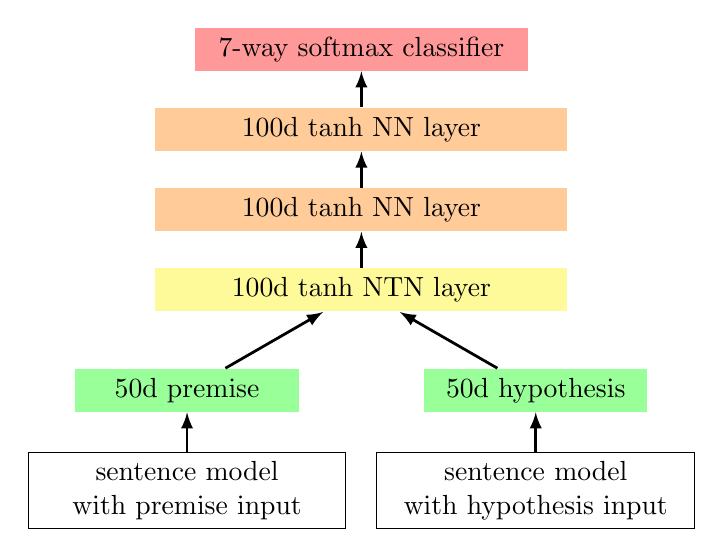
\begin{tikzpicture}
    \def\dx{21pt}
    \def\dy{29pt}

    \tikzstyle{label}=[text width=40mm,align=center]    
    \tikzstyle{softmax}=[fill=red!40,text width=40mm,align=center]
    \tikzstyle{preclass}=[fill=orange!40,text width=50mm,align=center]
    \tikzstyle{e}=[fill=green!40,text width=26mm,align=center]
    \tikzstyle{m}=[draw=black,text width=38mm,align=center]    
    
    \node[softmax]  (softmax) at (0*\dx,6*\dy) {7-way softmax classifier};
    \node[preclass]  (pc3) at (0*\dx,5*\dy) {100d $\tanh$ NN layer};
    \node[preclass]  (pc2) at (0*\dx,4*\dy) {100d $\tanh$ NN layer};
    \node[preclass,fill=yellow!40]  (pc1) at (0*\dx,3*\dy) {100d $\tanh$ NTN layer};
    \node[e]  (pe) at (-3*\dx,1.75*\dy) {50d premise};
    \node[e]  (he) at (3*\dx,1.75*\dy) {50d hypothesis};
    \node[m]  (pem) at (-3*\dx,0.5*\dy) {sentence model\\ with premise input};
    \node[m]  (hem) at (3*\dx,0.5*\dy) {sentence model\\ with hypothesis input};    
    
    \pgfsetarrowsend{latex}
    \tikzstyle{fwd} = [draw=black, line width=1pt]

          \draw [fwd] (pc3) -- (softmax);
          \draw [fwd] (pc2) -- (pc3);
          \draw [fwd] (pc1) -- (pc2);
          \draw [fwd] (pe) -- (pc1);
          \draw [fwd] (he) -- (pc1);
          \draw [fwd] (hem) -- (he);
          \draw [fwd] (pem) -- (pe);

  \end{tikzpicture}}
  
 \caption{The general architecture shared across models.}\label{fig:model:top}
  
\end{subfigure}

\begin{subfigure}[t]{0.45\textwidth}
  \centering
\scalebox{0.75}{
 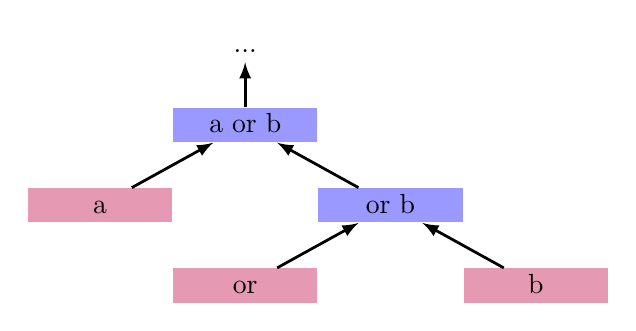
\begin{tikzpicture}
    \def\dx{21pt}
    \def\dy{29pt}


    \tikzstyle{word}=[fill=purple!40,text width=16mm,text height=2mm,align=center]
    \tikzstyle{node}=[fill=blue!40,text width=16mm,text height=2mm,align=center]
    \tikzstyle{empty}=[fill=blue!0,text width=8mm,text height=2mm,align=center]

    \node[empty]  (null) at (0*\dx,7*\dy) {...};
    \node[node]  (aorb) at (0*\dx,6*\dy) {a or b};
    \node[word]  (a) at (-2.5*\dx,5*\dy) {a};
    \node[node]  (orb) at (2.5*\dx,5*\dy) {or b};
    \node[word]  (or) at (0*\dx,4*\dy) {or};
    \node[word]  (b) at (5*\dx,4*\dy) {b};
    
    
    \pgfsetarrowsend{latex}
    \tikzstyle{fwd} = [draw=black, line width=1pt]

          \draw [fwd] (or) -- (orb);
          \draw [fwd] (b) -- (orb);
          \draw [fwd] (a) -- (aorb);
          \draw [fwd] (orb) -- (aorb);
          \draw [fwd] (aorb) -- (null);
  \end{tikzpicture}}
  
     \caption{The architecture for the TreeRNN and TreeRNTN sentence models. Terminal nodes are learned embeddings and nonterminal nodes are either NN or NTN layers with $\tanh$ nonlinearities.}\label{fig:model:tree}
  
  \end{subfigure}
 \vspace{0.5cm}
  
\begin{subfigure}[t]{0.45\textwidth}
  \centering
\scalebox{0.75}{
 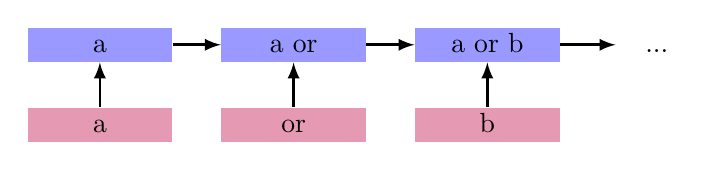
\begin{tikzpicture}
    \def\dx{35pt}
    \def\dy{29pt}


    \tikzstyle{word}=[fill=purple!40,text width=16mm,text height=2mm,align=center]
    \tikzstyle{node}=[fill=blue!40,text width=16mm,text height=2mm,align=center]
    \tikzstyle{empty}=[fill=blue!0,text width=8mm,text height=2mm,align=center]

    \node[word]  (a) at (-3*\dx,1*\dy) {a};
    \node[node]  (aN) at (-3*\dx,2*\dy) {a};
    
    \node[word]  (or) at (-1*\dx,1*\dy) {or};
    \node[node]  (orN) at (-1*\dx,2*\dy) {a or};
    
    \node[word]  (b) at (1*\dx,1*\dy) {b};
    \node[node]  (bN) at (1*\dx,2*\dy) {a or b}; 
    
    \node[empty]  (nullN) at (2.75*\dx,2*\dy) {...}; 
    
    \pgfsetarrowsend{latex}
    \tikzstyle{fwd} = [draw=black, line width=1pt]

          \draw [fwd] (or) -- (orN);
          \draw [fwd] (b) -- (bN);
          \draw [fwd] (a) -- (aN);
          \draw [fwd] (aN) -- (orN);
          \draw [fwd] (orN) -- (bN);
          \draw [fwd] (bN) -- (nullN);
          
  \end{tikzpicture}}
  
   \caption{The architecture for the LSTM sentence model. Nodes in the lower row are learned embeddings and nodes on the upper row are LSTM units.}\label{fig:model:seq}
  
    \end{subfigure}
  \caption{In our model, two copies of a sentence model---based on either tree (b) or sequence (c) models---encode the two input sentences. A multilayer classifier component (a) then uses the resulting vectors to predict a label that reflects the logical relationship between the two sentences.}
  \label{sample-figure}
\end{figure*}


\paragraph{Classifier}
The classifier component of the model consists of a combining layer which takes the two sentence representations as inputs, followed by two neural network layers, then a softmax classifier.
For the combining layer, we use a neural tensor network (NTN, \cite{chen2013learning}) layer, which sums the output of a plain recursive/recurrent neural network layer with a vector computed using two multiplications with a learned (full rank) third-order tensor parameter:
\begin{gather} 
\label{TreeRNN}
\vec{y}_{\textit{NN}} = \tanh(\mathbf{M} \colvec{2}{\vec{x}^{(l)}}{\vec{x}^{(r)}} + \vec{b}\,) \\
\label{TreeRNTN} 
\vec{y}_{\textit{NTN}} = \vec{y}_{\textit{NN}} + \tanh(\vec{x}^{(l)T} \mathbf{T}^{[1 \ldots n]} \vec{x}^{(r)})
\end{gather} 

Our model is largely identical to the model from \newcite{Bowman:Potts:Manning:2014}, but adds the two additional $\tanh$ NN layers, which we found help performance across the board, and also uses the NTN combination layer when evaluating all four models, rather than just the TreeRNTN model, so as to ensure that the sentence models are compared in as similar a setting as possible.

We only study models that encode entire sentences in fixed length vectors, and we set aside models with attention \cite{bahdanau2014neural}, a technique which gives the downstream model (here, the classifier) the potential to access each input token individually through a soft content addressing system. While attention simplifies the problem of learning complex correspondences between input and output, there is no apparent reason to believe that it should improve or harm a model's ability to track structural information like a given token's position in a tree. As such, we expect our results to reflect the same basic behaviors that would be seen in attention-based models.

\paragraph{Sentence models}
The sentence encoding component of the model transforms the (learned) embeddings of the input words for each sentence into a single vector representing that sentence. We experiment with tree-structured models (Figure~\ref{fig:model:tree}) with TreeRNN (eqn.~\ref{TreeRNN}), TreeRNTN (eqn.~\ref{TreeRNTN}), and TreeLSTM \cite{tai2015improved} activation functions. In addition, we use a sequence model (Figure~\ref{fig:model:seq}) with an LSTM activation function \cite{hochreiter1997long} implemented as in \newcite{zaremba2015recurrent}. In experiments with a simpler non-LSTM RNN sequence model, the model tended to badly underfit the training data, and those results are not included here.

\paragraph{Training} We randomly initialize all embeddings and layer parameters, and train them using minibatch stochastic gradient descent with AdaDelta \cite{zeiler2012adadelta} learning rates. Our objective is the standard negative log likelihood classification objective with L2 regularization (tuned on a separate train/test split). All models were trained for 100 epochs, after which all had largely converged without significantly declining from their peak performances.

\section{General discussion}\label{sec:discussion}

This paper evaluated two recursive models on a series of three increasingly
challenging interpretive tasks involving natural language inference:
the core labelal algebra of natural logic with entailment and
exclusion; recursive propositional logic structures; and statements
involving quantification and negation. The results suggest that RNTNs,
but not plain RNNs, have the capacity to meet the challenges of these
tasks with reasonably-sized training sets. These positive results are
promising for the future of learned representation models in the
applied modeling of compositional semantics.

Of course, challenges remain. In terms of our experimental data, even
the RNTN falls short of perfection in our more complex tasks, with
performance falling off steadily as the depth of recursion grows. It
remains to be seen whether these deficiencies can be overcome with
improvements to the model, the optimization procedures, or the
linguistic representations
\cite{sochergrounded,kalchbrenner2014convolutional}. In addition,
there remain subtle questions about how to fairly assess whether these
models have truly generalized in the way we want them to. There is a
constant tension between showing the models training data that gives
them a chance to learn the target logical functions and revealing the
answer to them in a way that leads to overfitting. The underlying
logical theories provide only limited guidance on this point.
%
%, and the fact that there is a finite universe of possible
%  expressions makes his an unavoidable issue. 
%
%  CP: I don't understand the above. It is false if taken literally;
%  our PL generates an infinte number of formulae.
%
Finally, we have only scratched the surface of the logical complexity
of natural language; in future experiments, we hope to test sentences
with embedded quantifiers, multiple interacting quantifiers, relative
clauses, and other kinds of recursive structure. Nonetheless, the
rapid progress the field has made with these models in recent years
provides ample reason to be optimistic that they can be trained to
meet the challenges of natural language semantics.

% These experiments represent one of the first attempts to reproduce any large fragment of the behavior of a complex logic within a neural network model, and the first attempt that we are aware of to address either the encoding of lexical labels or the learning of recursive operators. This presents considerable challenges in evaluating the particular models that we choose, since we cannot rely on prior results to establish that any particular amount or type of training data is sufficient to teach any model the structure of the logic. The positive results that we have found, however, are extremely promising for the future of learned representation models in the applied modeling of meaning. We have seen that recursive neural tensor networks are able to encode lexical labels accurately and encode recursive operators. We have also seen that both RNNs and RNTNs are able to handle the meanings of quantifiers in an inference setting in at least some cases. 

% There is ample room to build on these results. In the interest of fully mirroring the capacity of existing natural logics in learned models, it would be valuable to extend these experiments to cover other ways in which meanings are encoded in natural language, including challenges such as reasoning over sentences with transitive verbs or relative clauses. In addition, it would be highly informative to compare these results on standard recursive neural networks with other proposed learned models for sentence meaning, such as dependency tree RNNs \cite{sochergrounded}, Belief Propagation RNNs (TODO: cite), or convolutional RNNs \cite{kalchbrenner2014convolutional}.



%\subsubsection*{Acknowledgments}

% We thank Jeffrey Pennington, Richard Socher, and audiences at CSLI, Nuance, and BayLearn, as well as Neha Nayak for developing the SICK collapsing technique.

\subsubsection*{Acknowledgments}

%
We gratefully acknowledge support from %
a Google Faculty Research Award, %
a gift from Bloomberg L.P., 
the Defense Advanced Research Projects Agency (DARPA) Deep Exploration and Filtering of Text (DEFT) Program under Air Force Research Laboratory (AFRL) contract no.~FA8750-13-2-0040,
the National Science Foundation under grant no.~IIS 1159679, and %
the Department of the Navy, Office of Naval Research, under grant no.~N00014-13-1-0287.
%
Any opinions, findings, and conclusions or recommendations expressed in this material are those of the authors and do not necessarily reflect the views of 
Google, 
Bloomberg L.P.,
DARPA,
AFRL
NSF, 
ONR, or 
the US government.

\bibliographystyle{unsrtnat}
\bibliography{MLSemantics} 

\end{document}
